\chapter[Second Hox data set]{Second Hox data set}

In order to increase confidence in the $g$-tensor solution of Table~6.1 an additional rotation set in two planes was performed on the same crystal. The crystal was removed from the resonator and rotated arbitrarily within the micro-helix to obtain the secondary dataset. The data was then fit assuming the rotation was only around the L$_3$ axis. 

\begin{figure}[ht]
\centering
 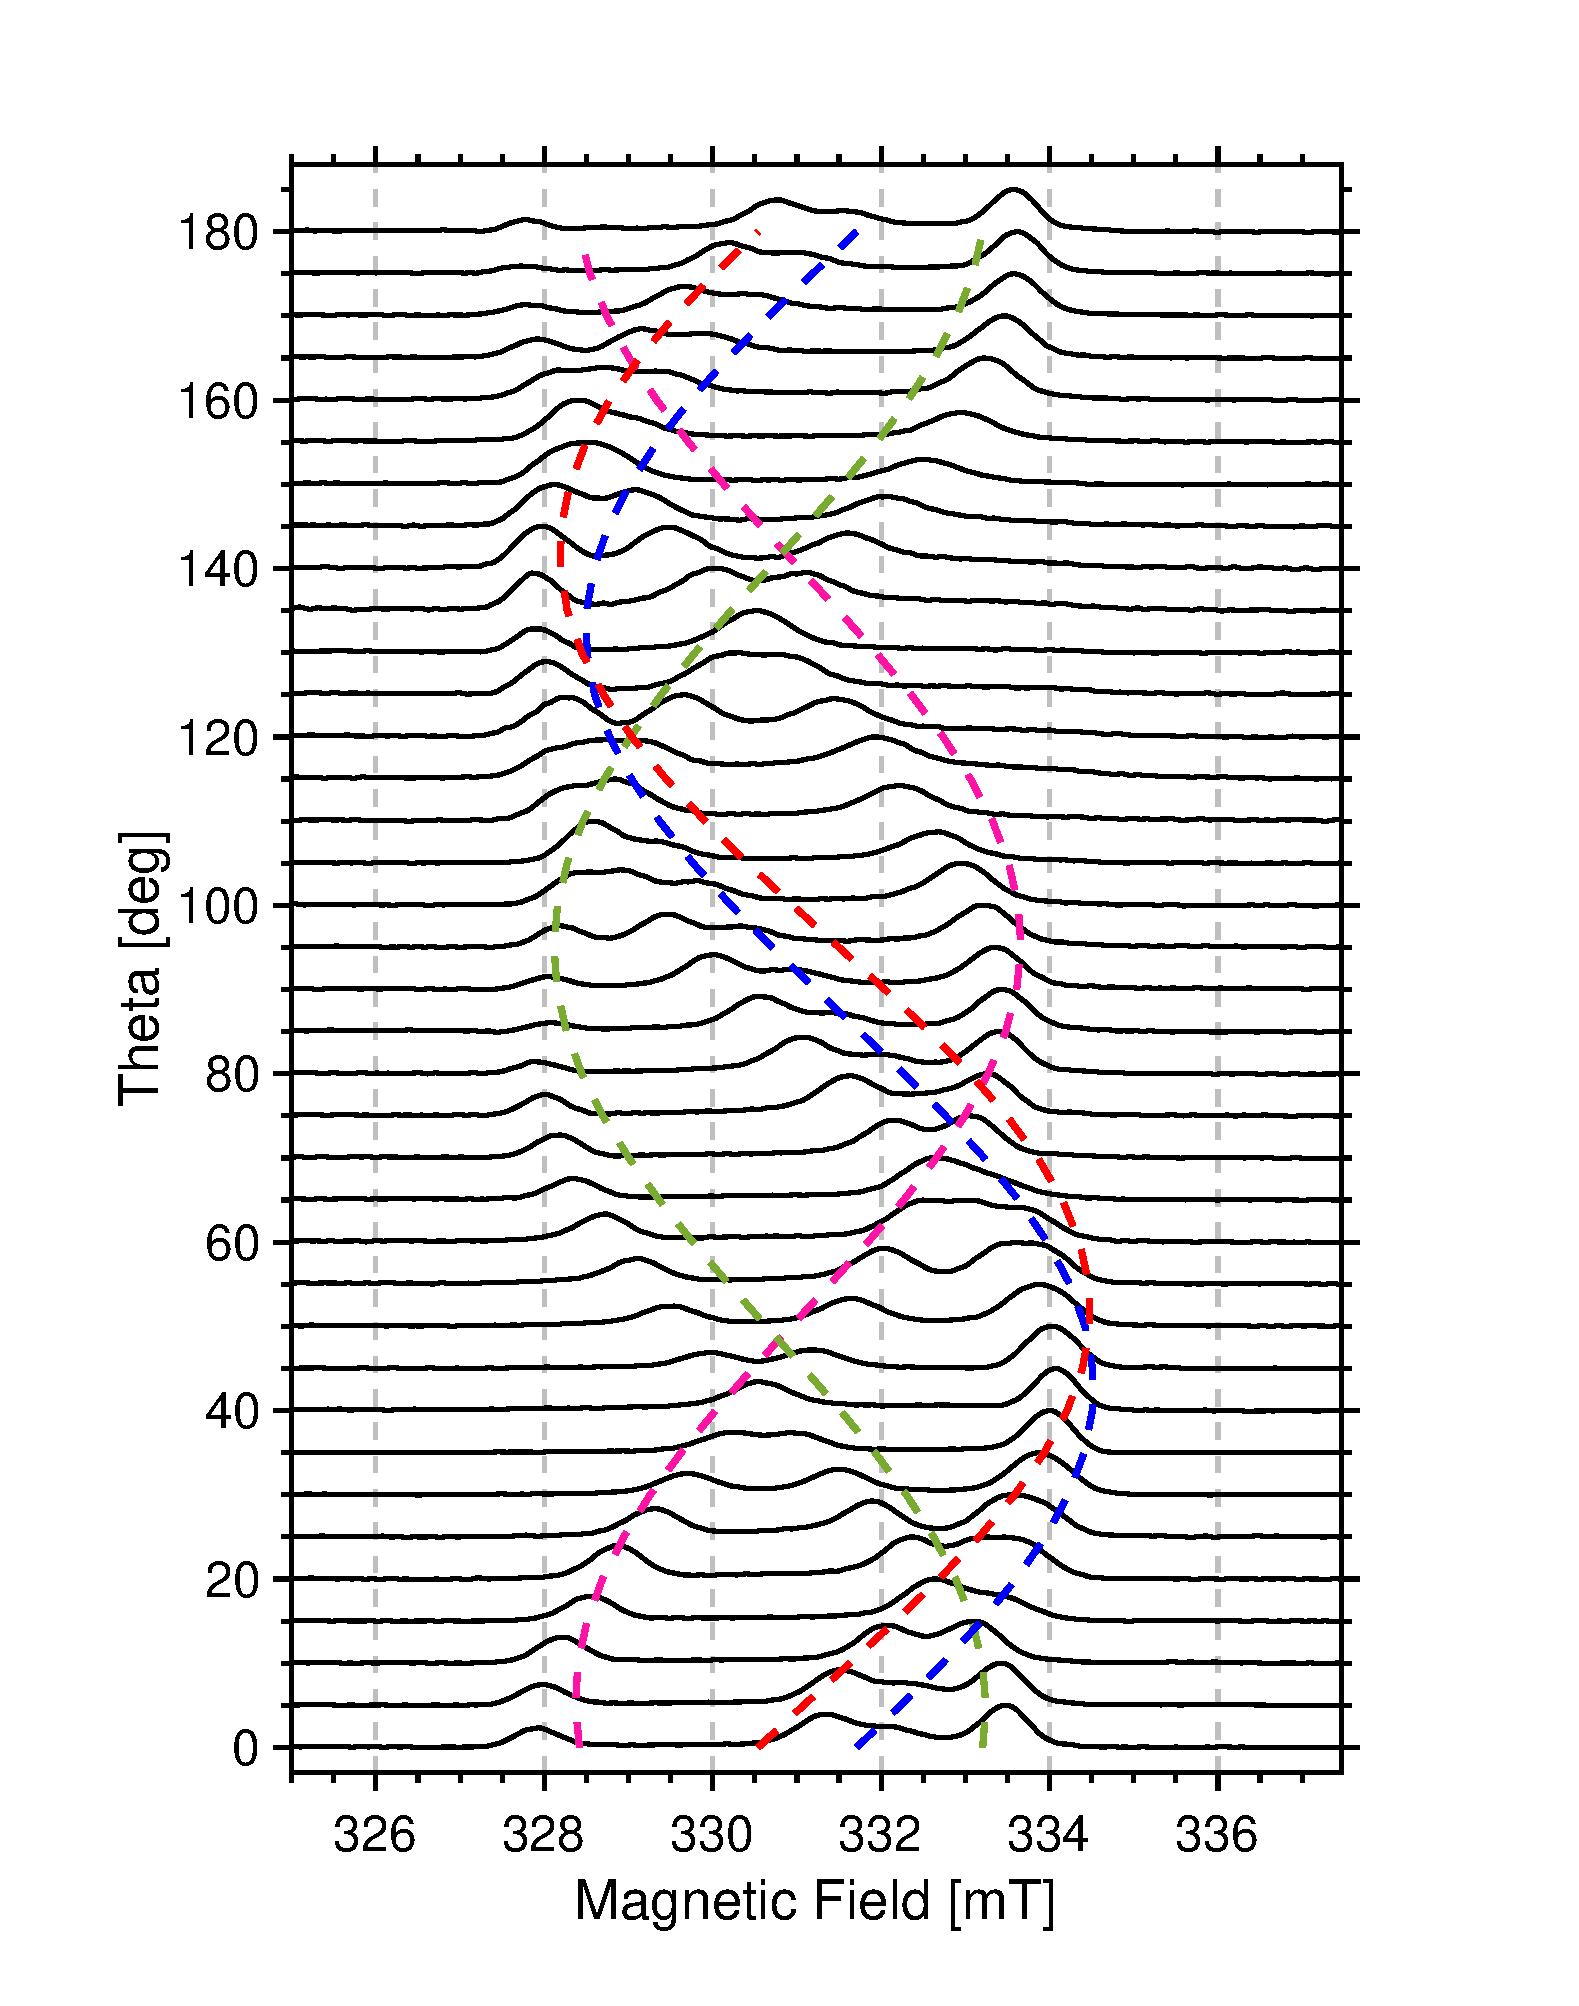
\includegraphics[width=0.8\textwidth]{Kapitel/Appendix/RotateCrystal180.eps}\label{fig-app:Rotate}
 \caption[Single Crystal Roadmap around L$_3$ axis]{Single-crystal ESE data with resonance roadmap rotating the crystal around the L$_3$ axis with the helix axis parallel to the L$_3$ axis. Setup shown in Fig.~\ref{fig:RotateMe}A} 
\end{figure} 

\begin{figure}[ht]
\centering
 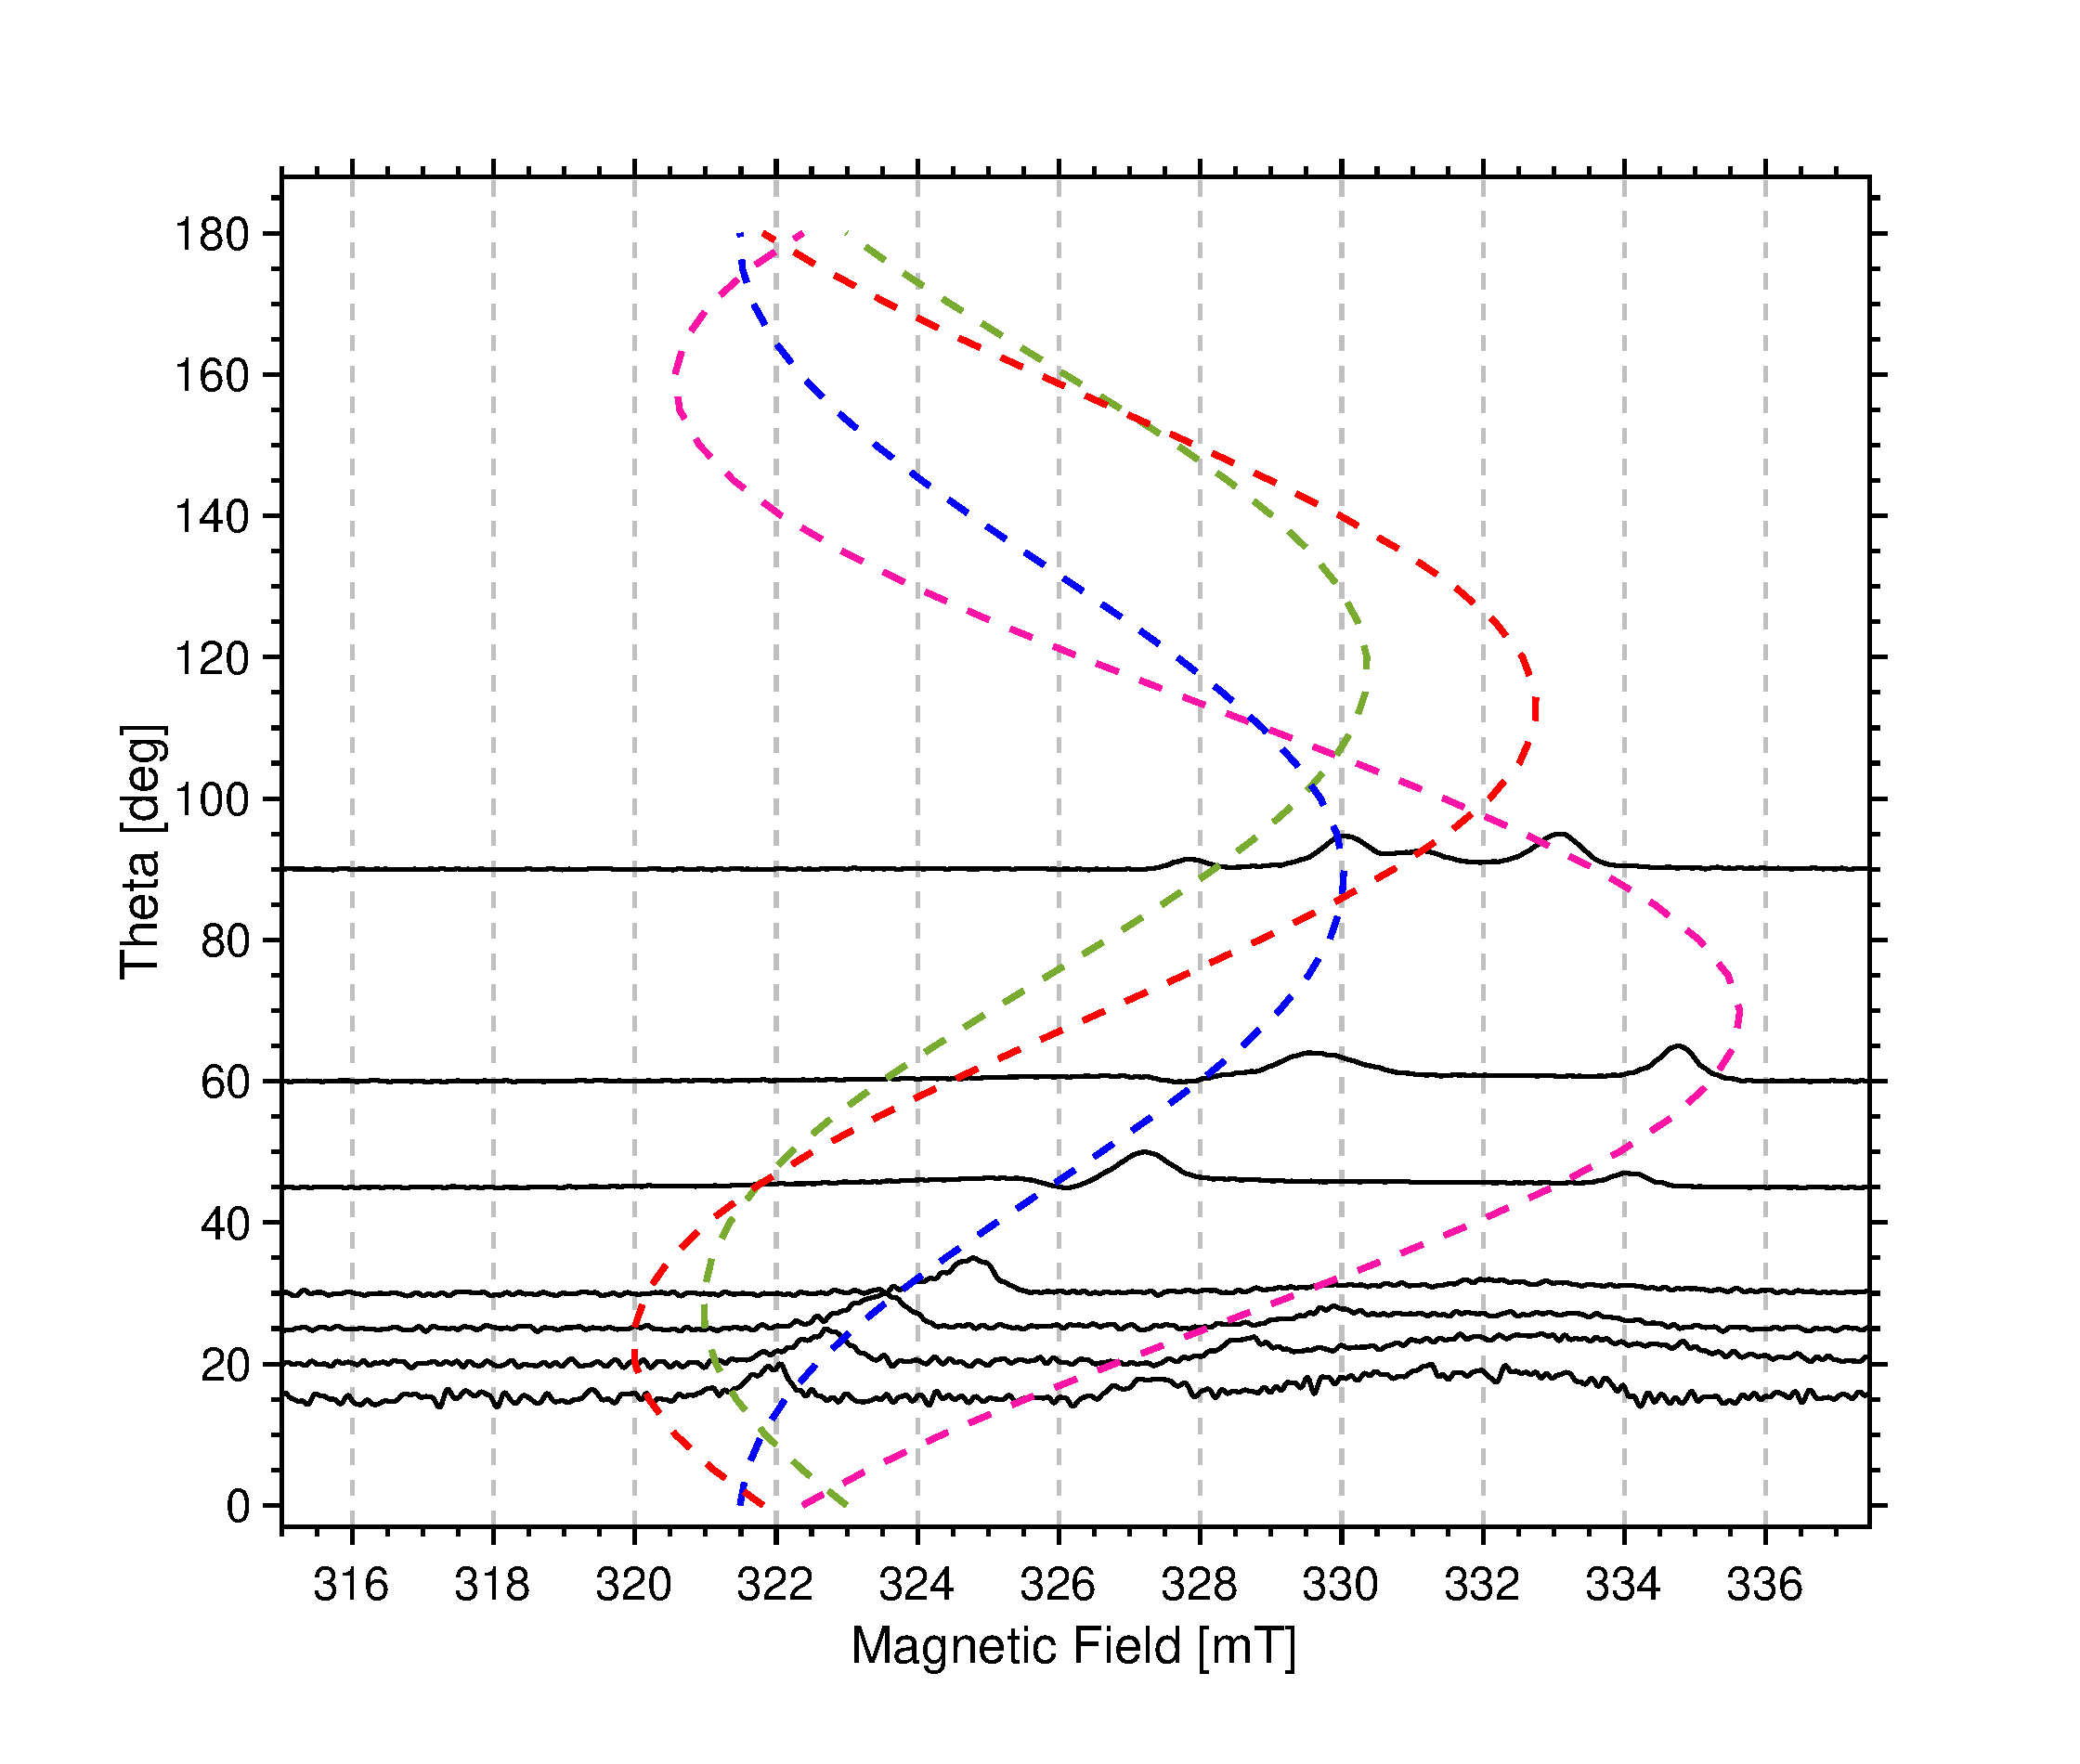
\includegraphics[width=0.8\textwidth]{Kapitel/Appendix/RotateCrystal.eps}
 \caption[Single Crystal Roadmap around L$_3$ axis rotated B$_1$ to the L$_2$ axis.]{Single-crystal ESE data with resonance roadmap rotating the crystal around the L$_3$ axis with the helix axis parallel to the L$_2$ axis. Setup shown in Fig.~\ref{fig:RotateMe}B} 
\end{figure} \label{fig-app:Rotate90}

